\begin{question}
\noindent Shape $T$ is drawn on the grid below. The point marked with a dot is the centre of rotation, $(1,1)$.

\begin{center}
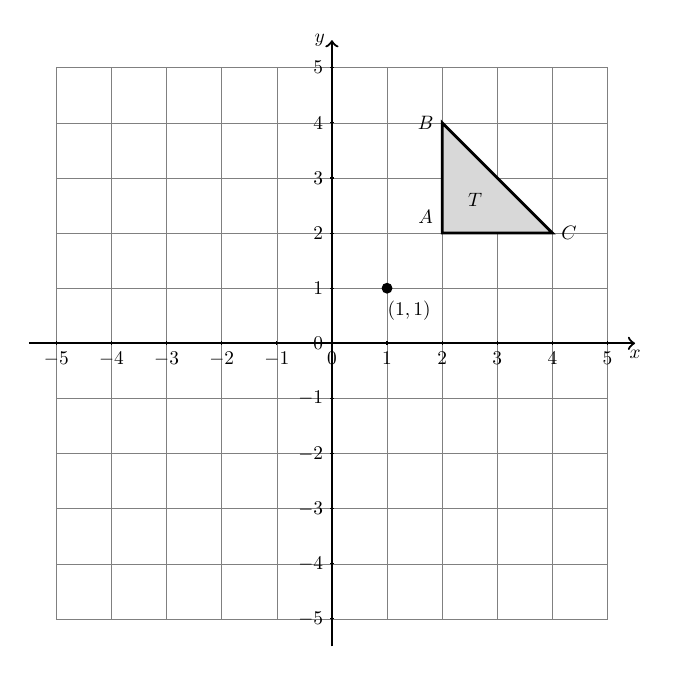
\begin{tikzpicture}[scale=0.7, transform shape]
    \def\axisLimit{5}

    \definecolor{borderColour}{HTML}{000000}
    \definecolor{fillColour}{HTML}{D8D8D8}

    % Grid
    \draw[step=1cm,gray,very thin] (-\axisLimit,-\axisLimit) grid (\axisLimit,\axisLimit);

    % Axes
    \draw[thick,->] (-\axisLimit-0.5,0) -- (\axisLimit+0.5,0) node[anchor=north] {$x$};
    \draw[thick,->] (0,-\axisLimit-0.5) -- (0,\axisLimit+0.5) node[anchor=east] {$y$};

    % Axis labels
    \foreach \x in {-\axisLimit,...,\axisLimit}
        \draw (\x cm,1pt) -- (\x cm,-1pt) node[anchor=north] {$\x$};
    \foreach \y in {-\axisLimit,...,\axisLimit}
        \draw (1pt,\y cm) -- (-1pt,\y cm) node[anchor=east] {$\y$};

    % Centre of rotation
    \coordinate (center) at (1,1);
    \filldraw[black] (center) circle (2.5pt);
    \node at (1.4,0.6) {$(1,1)$};

    % Shape T: right-angled triangle
    \coordinate (A) at (2,2);
    \coordinate (B) at (2,4);
    \coordinate (C) at (4,2);

    \filldraw[fill=fillColour, draw=borderColour, line width=1pt] (A) -- (B) -- (C) -- cycle;
    \node at (1.7,2.3) {$A$};
    \node at (1.7,4) {$B$};
    \node at (4.3,2) {$C$};
    \node at (2.6,2.6) {$T$};

\end{tikzpicture}
\end{center}

\noindent Rotate shape $T$ $90^\circ$ clockwise about the point $(1,1)$.

\noindent Draw the image of shape $T$ on a grid and label it $T'$, stating the coordinates of the image of each vertex.

\vspace{5cm}

\begin{flushright}
\answerplain{3}
\end{flushright}
\end{question}
